\documentclass[11pt,onecolumn]{article}
\usepackage[margin=1in]{geometry}
\usepackage{graphicx}
\usepackage{float}
\usepackage{siunitx}
\usepackage[settings]{markdown}
\usepackage{hyperref}
\usepackage{breakurl}
\usepackage{titlesec}
\usepackage{authblk}
\usepackage{abstract}

\graphicspath{ {./content/} }

% Attempt to mimic IEEEtran styling
\usepackage{times}
\usepackage{mathptmx}
\usepackage{microtype}

% Adjust section formatting to be more like IEEEtran
\titleformat{\section}{\normalfont\Large\bfseries}{\thesection.}{1em}{}
\titleformat{\subsection}{\normalfont\large\bfseries}{\thesubsection.}{1em}{}

\title{A Comparative Study of OpenCL and XRT Performance for Data Transfers on Xilinx FPGA}

\author[]{Qasim Li}
\affil[]{McGill University}
\affil[]{Supervised by Christophe Dubach}

\date{Created August 20, 2024; revised August 30, 2024}

\begin{document}

\maketitle

\section{Introduction}
This test suite is used for benchmarking the bandwidth and latency of data transfers between the cpu and global memory. It focuses on benchmarking the transfer speeds of various APIs (XRT API and OpenCL/OCL) between the host and the FPGA board. \\

In this experiment, the goal is to find out the overhead of using each of the APIs, whether one API gives a speed advantage over the other. This is done by transferring data between the host and the fpga board, starting from the lowest data transfer size possible and increasing the size by powers of two.


\section{Background}
In a typical Vitis platform, a host system (typically a CPU) interacts with an FPGA board to accelerate specific tasks. The FPGA has access to global memory (gmem, the ram on the fpga board), which serves as a shared space for data exchange between the host and FPGA. \\

Developers can use either the OpenCL API or the Xilinx Runtime (XRT) API to manage this interaction. These APIs allow the host to control the FPGA, load kernels (specialized functions implemented on the FPGA), transfer data to and from the global memory, and synchronize operations. \\

OpenCL provides a more generalized, high-level interface, while XRT offers FPGA-specific, lower-level control. This setup enables efficient offloading of computationally intensive tasks from the host to the FPGA, leveraging hardware acceleration while maintaining a flexible software development environment.
\section{Overview}

This study aims to comprehensively evaluate and compare the performance of OpenCL and XRT APIs for data transfers between the host CPU and FPGA global memory. Our primary objectives are to: \\

\begin{enumerate}
    \item Determine if there's a significant performance difference between OpenCL and XRT APIs for data transfers.
    \item Understand how data transfer sizes affect the performance of each API.
    \item Investigate the impact of consecutive READ/WRITE operations on transfer speeds.
    \item Identify scenarios where one API might be preferable over the other.
\end{enumerate}

To achieve these goals, we will conduct a series of benchmarks that measure: \\
\begin{enumerate}
    \item READ and WRITE speeds from CPU to global memory using both APIs.
    \item Performance of consecutive read and write operations.
    \item Transfer speeds across a wide range of data sizes, from very small to very large, incrementing by powers of 2.
\end{enumerate}

\begin{figure}[H]
    \centering
    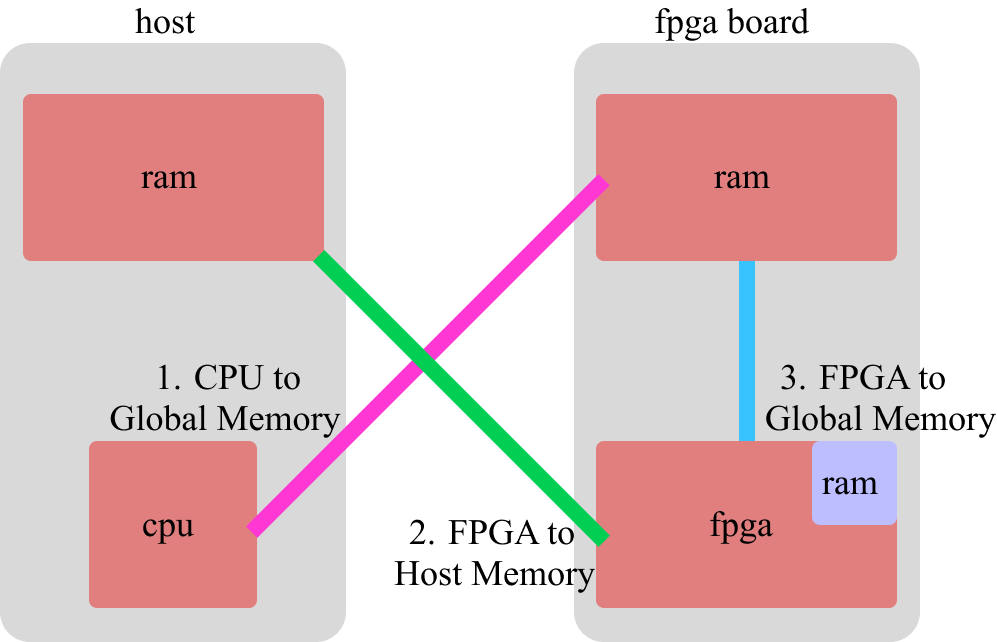
\includegraphics[width=0.6\linewidth]{content/cpu_fpga_board_layout.png}
    \caption{Layout of the Host and FPGA Board and Data Transfer Paths.}
    \label{fig:enter-label}
\end{figure}

There are 3 main ways to transfer data, referencing Fig. 1. 
\begin{enumerate}
    \item CPU READ/WRITE Global Memory

    One main way to transfer data to and from the FPGA is through the global memory (gmem). In this case, the Host will take data from it's own memory and allocate space and copy it over to the gmem. To perform this transfer, you can either use the OpenCL or XRT API. This test is used to discover whether one API has a data transfer speed advantage over the other, if at all any.

    \item FPGA READ/WRITE Global Memory - \texttt{NOT CURRENTLY SUPPORTED}

    In order for the FPGA to communicate with the Host using the previous method, it needs to read and write to the gmem. This tests is mainly used to benchmark the access speeds of the FPGA to the gmem.
    
    \item FPGA READ/WRITE Host Memory - \texttt{NOT CURRENTLY SUPPORTED}

    Another method for the Host and the FPGA to communicate is to have the FPGA read and write directly to the Host memory. This method is simpler as it removes the need to synchronise the read and writes of the Host and FPGA like in the first method. By comparing the data transfer speeds of this method to that of the total of the Host to gmem and FPGA to gmem speeds, the optimal method of data transfers can be found. \\
\end{enumerate}

We will analyze the results to identify performance trends, peak transfer rates, and any potential bottlenecks or overhead issues. This analysis will provide valuable insights for developers working on FPGA-accelerated applications, helping them make informed decisions about which API to use based on their specific use cases and data transfer requirements.

The initial platform that this was tested on \texttt{Alveo U200}, supported this feature. However, the FPGA board that AWS F1 instances use \texttt{Xilinx UltraScale Plus FPGA} was not compatible with test including the FPGA. Alternative methods are currently being investigated. \\
\section{Environment}

For these benchmark tests, the emulation tests were ran on a \texttt{AWS EC2 z1d.2xlarge} instance while the hardware tests were ran on a \texttt{AWS EC2 f1.2xlarge} instance. The FPGA or target platform for those 2 instances were ran on a \texttt{Xilinx UltraScale Plus FPGA}.
\section{Benchmarks}

Below outlines the results from the hardware (on FPGA) benchmarking tests and comparison to their results from the hardware emulation benchmarking tests. On the left side lies the hardware results and left is the emulation results. The emulation results are taken from running the benchmark tests on AWS EC2 z1d.2xlarge instance and the hardware results are taken from a AWS EC2 f1.2xlarge instance. This is done so that the target platform (FPGA board) will be the same in emulation and hardware for closest comparison.\\

The purpose of these benchmarks is the measure the throughput of the data transmissions. That is, the rate at which the data of different sizes arrives at it's destination successfully. On the y-axis, it displays the transfer speeds in GB/s and on the x-axis, it displays the transfer size in bytes. The x-axis is graphed on a log time scale due to the fact that the data sizes are increased by powers of 2 each iteration. \\

There are 4 total types of graph for each of the host APIs: READ, WRITE, READ RW, and WRITE RW. The first 2, READ and WRITE are just for single data transfers and READ RW, and WRITE RW benchmarks data transfers when consecutive READ \& WRITE data transfers are ran continuously. This is done to see if consecutive READ/WRITEs will throttle the throughput. \\

You may notice that the results for \texttt{FPGA to Host Memory} is missing. This is because while it compiled and ran fine on \texttt{Alveo U200}'s hardware emulation tests, AWS EC2 F1 instances use \texttt{Xilinx UltraScale Plus FPGA}s, which does not support the current method used to test FPGA READ/WRITE from Host Memory, therefore the results are omitted. \\

Furthermore, there seems to be a bug with the way AWS handles hardware compilation and execution, sometimes omitting necessary data such as \texttt{timeline\_kernels.csv} after execution, which appeared in the emulation tests performed on both the \texttt{Alveo U200} and \texttt{Xilinx UltraScale Plus FPGA}. There is possibility that AWS does not send data back from the FPGA after a execution is ran, preventing some XRT Runtime flags to be obsolete. Thus, the \texttt{FPGA to Global  Memory} results are also omitted. \\

Methods to fix the previous 2 problems are currently being investigated. \\

\begin{figure}[H]
    \centering
    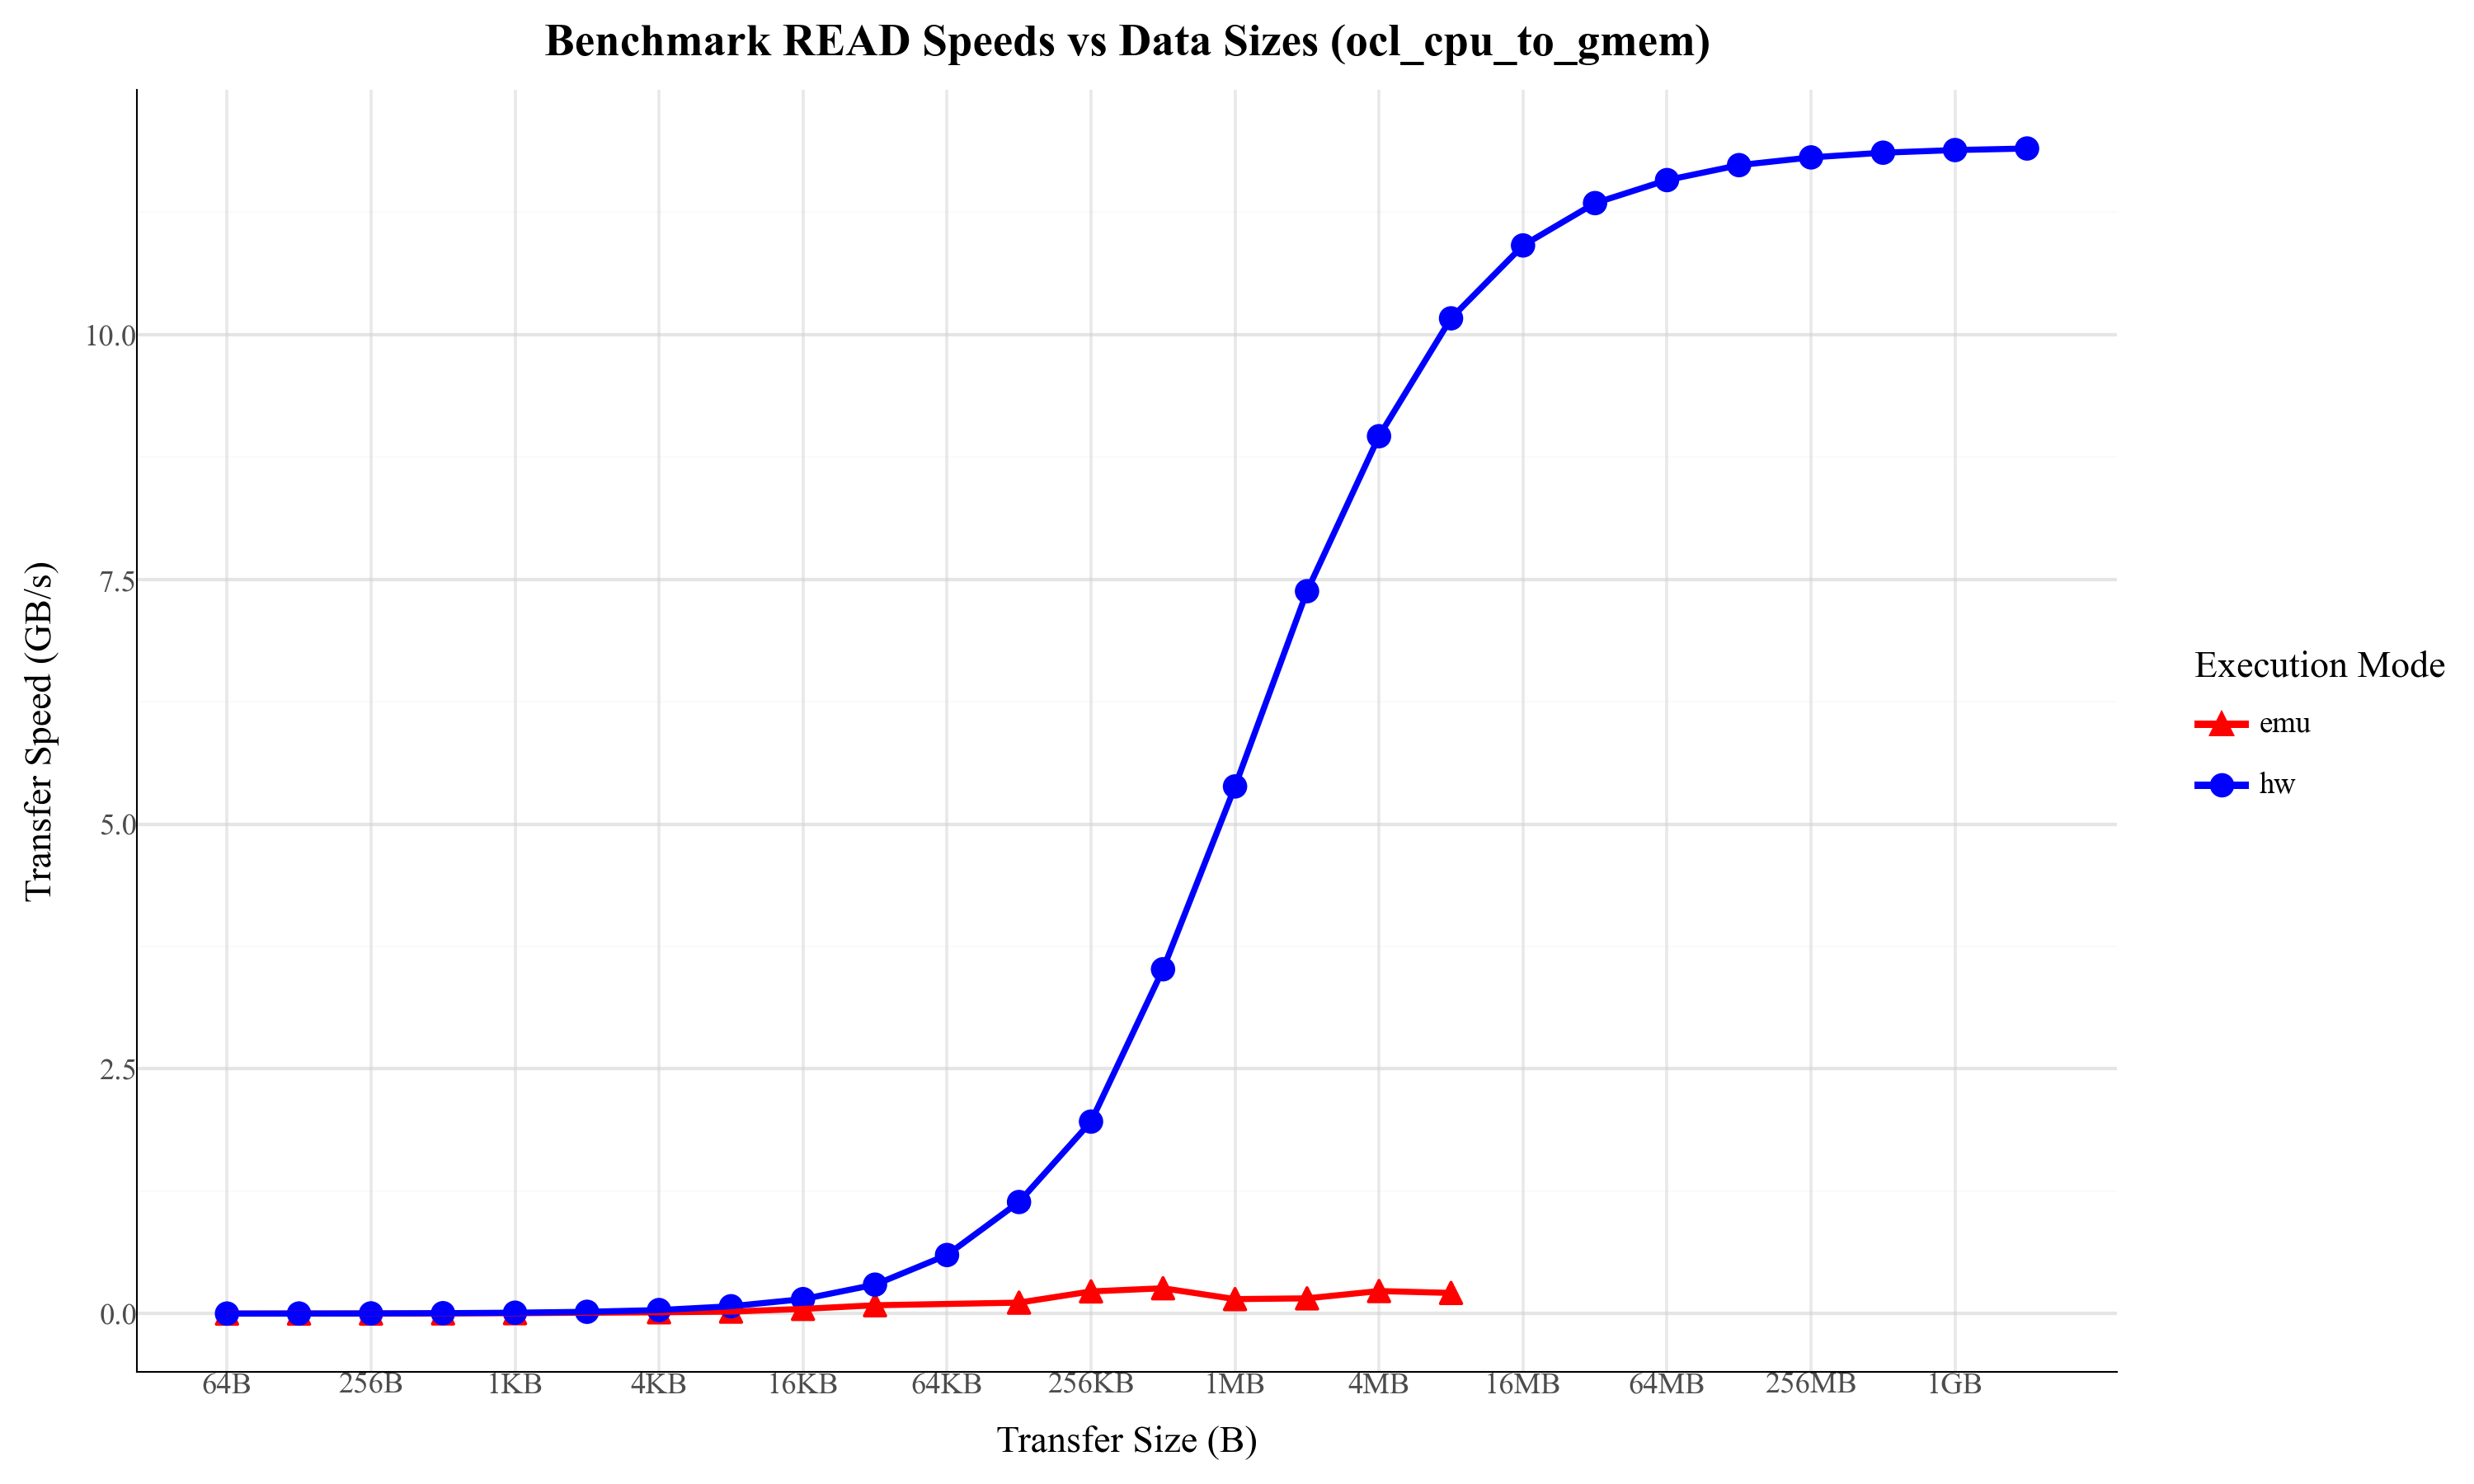
\includegraphics[width=0.9\linewidth]{content/ocl_cpu_to_gmem_READ.png}
    \caption{Log10 Graph of Data READ Speeds Comparison from CPU to GMEM for HW and EMU using OCL.}
    \label{fig:enter-label}
\end{figure}

\begin{figure}[H]
    \centering
    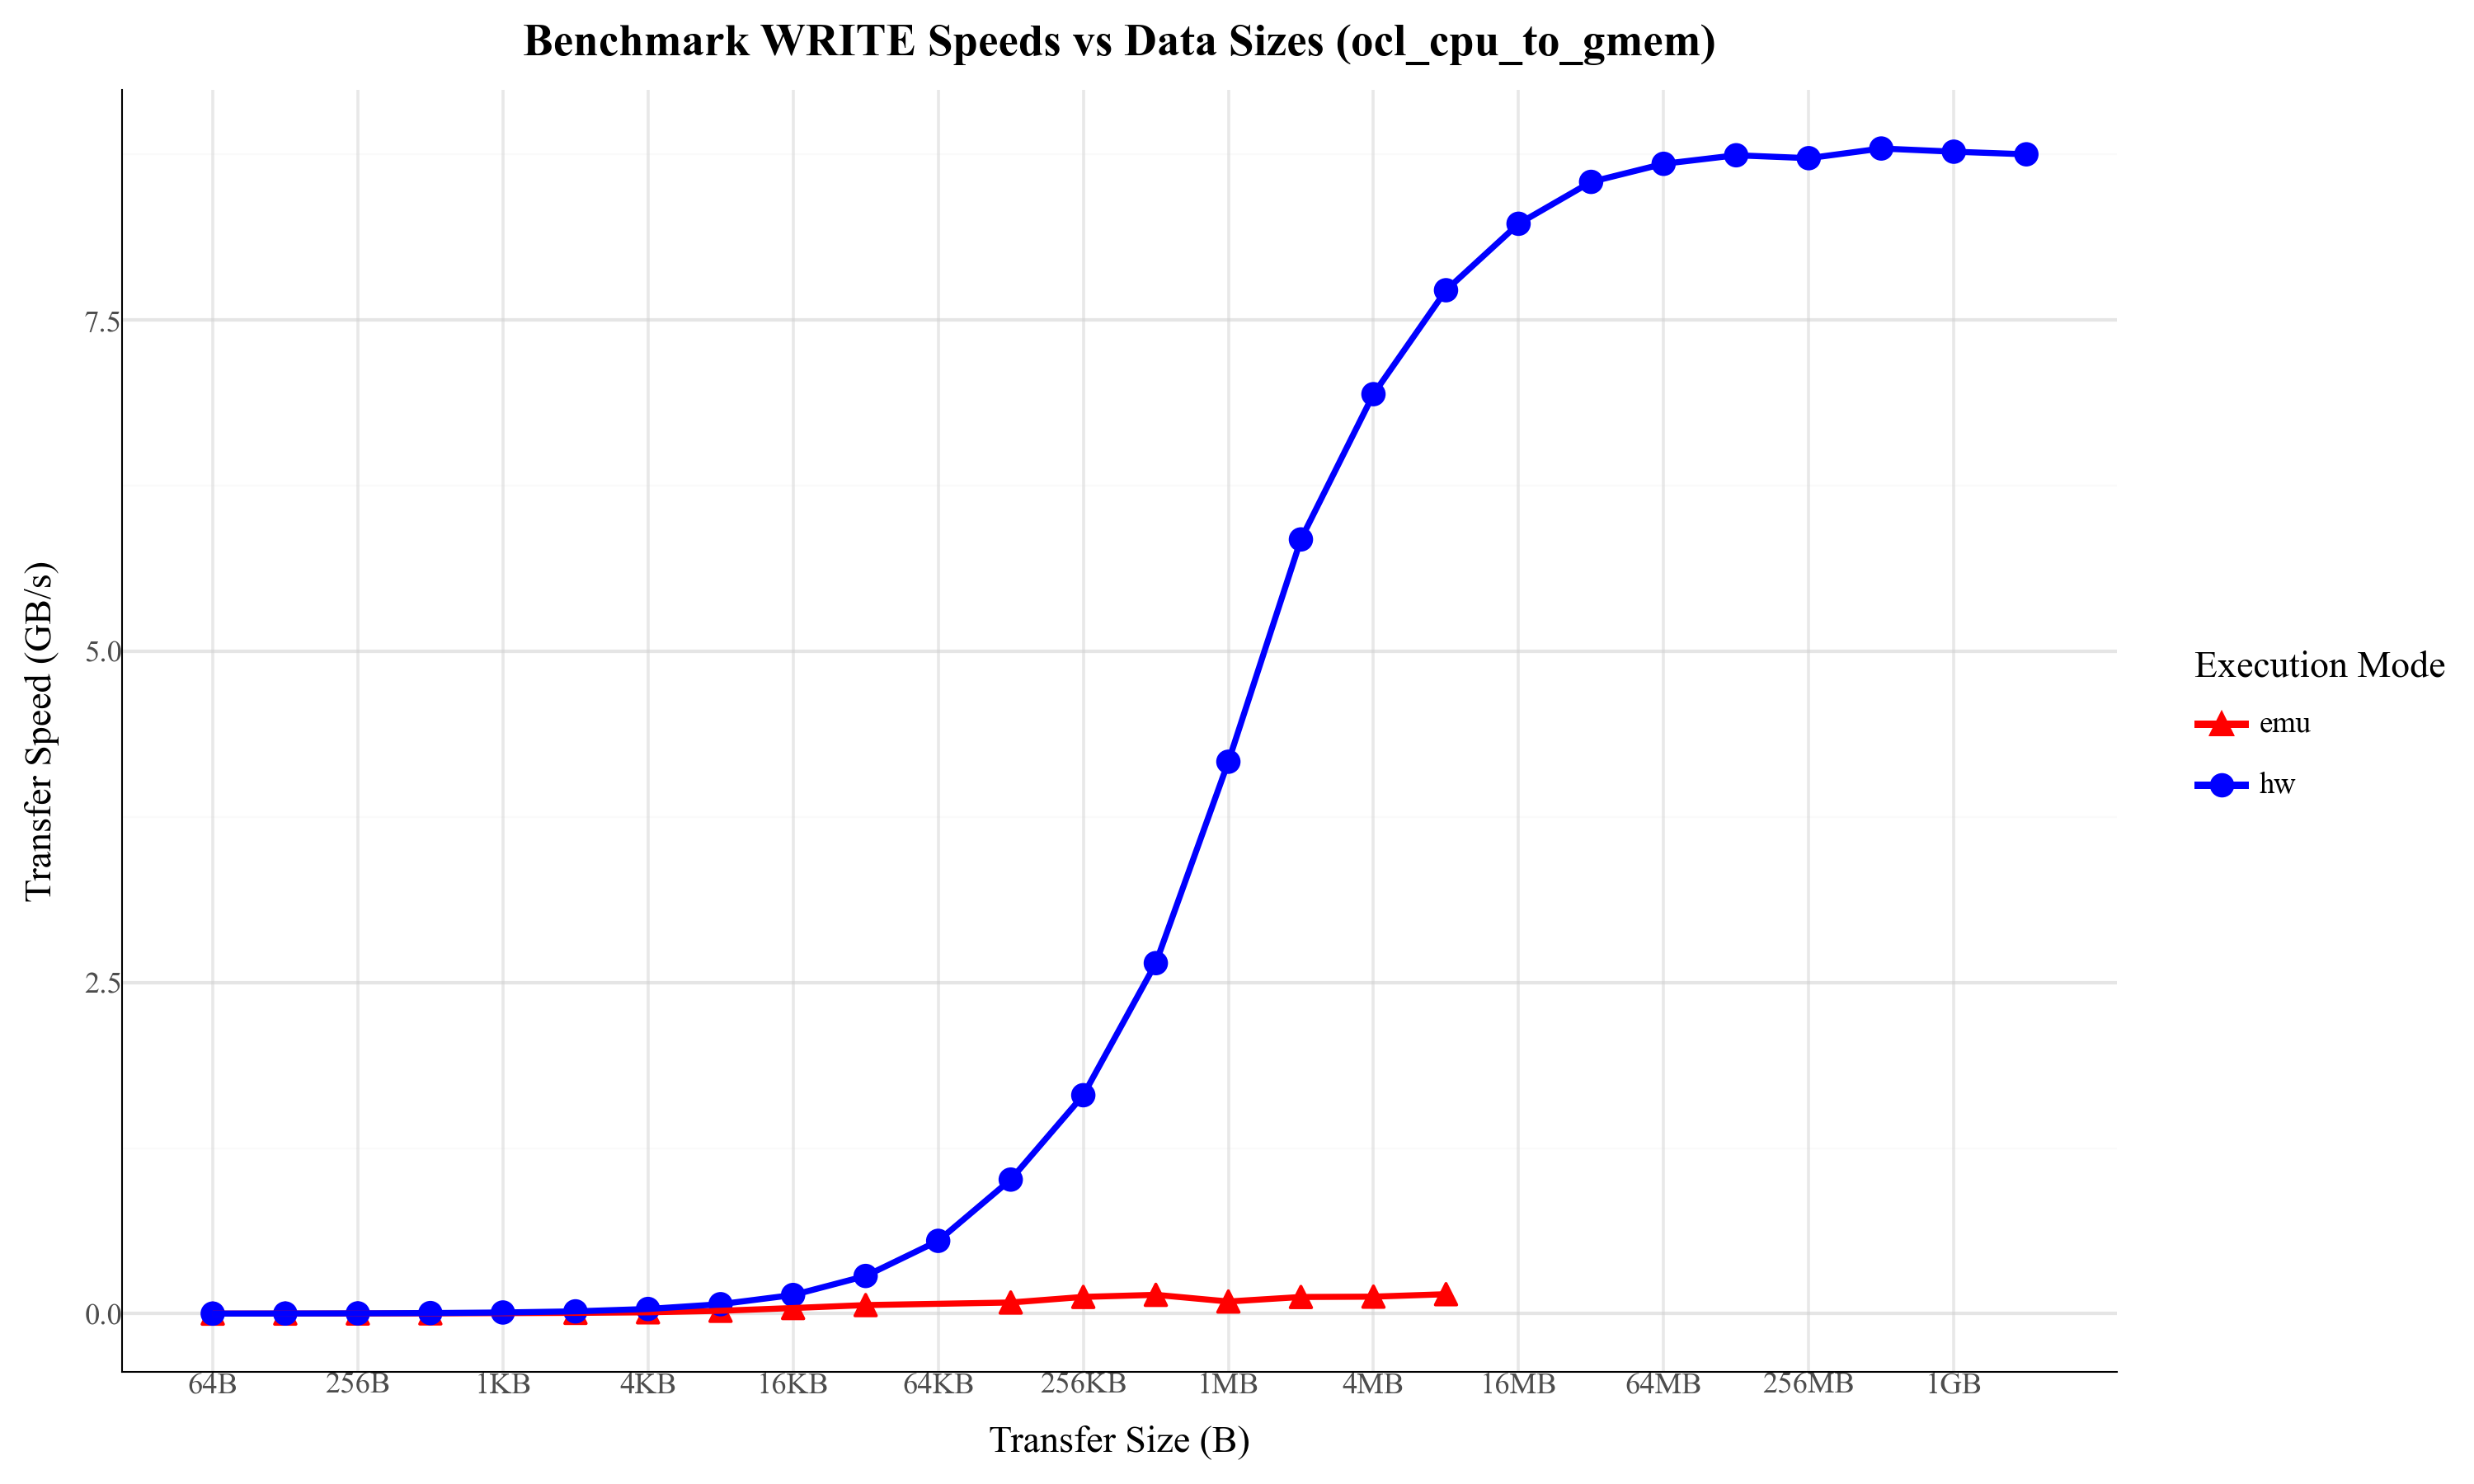
\includegraphics[width=0.9\linewidth]{content/ocl_cpu_to_gmem_WRITE.png}
    \caption{Log10 Graph of Data WRITE Speeds Comparison from CPU to GMEM for HW and EMU using OCL.}
    \label{fig:enter-label}
\end{figure}

\begin{figure}[H]
    \centering
    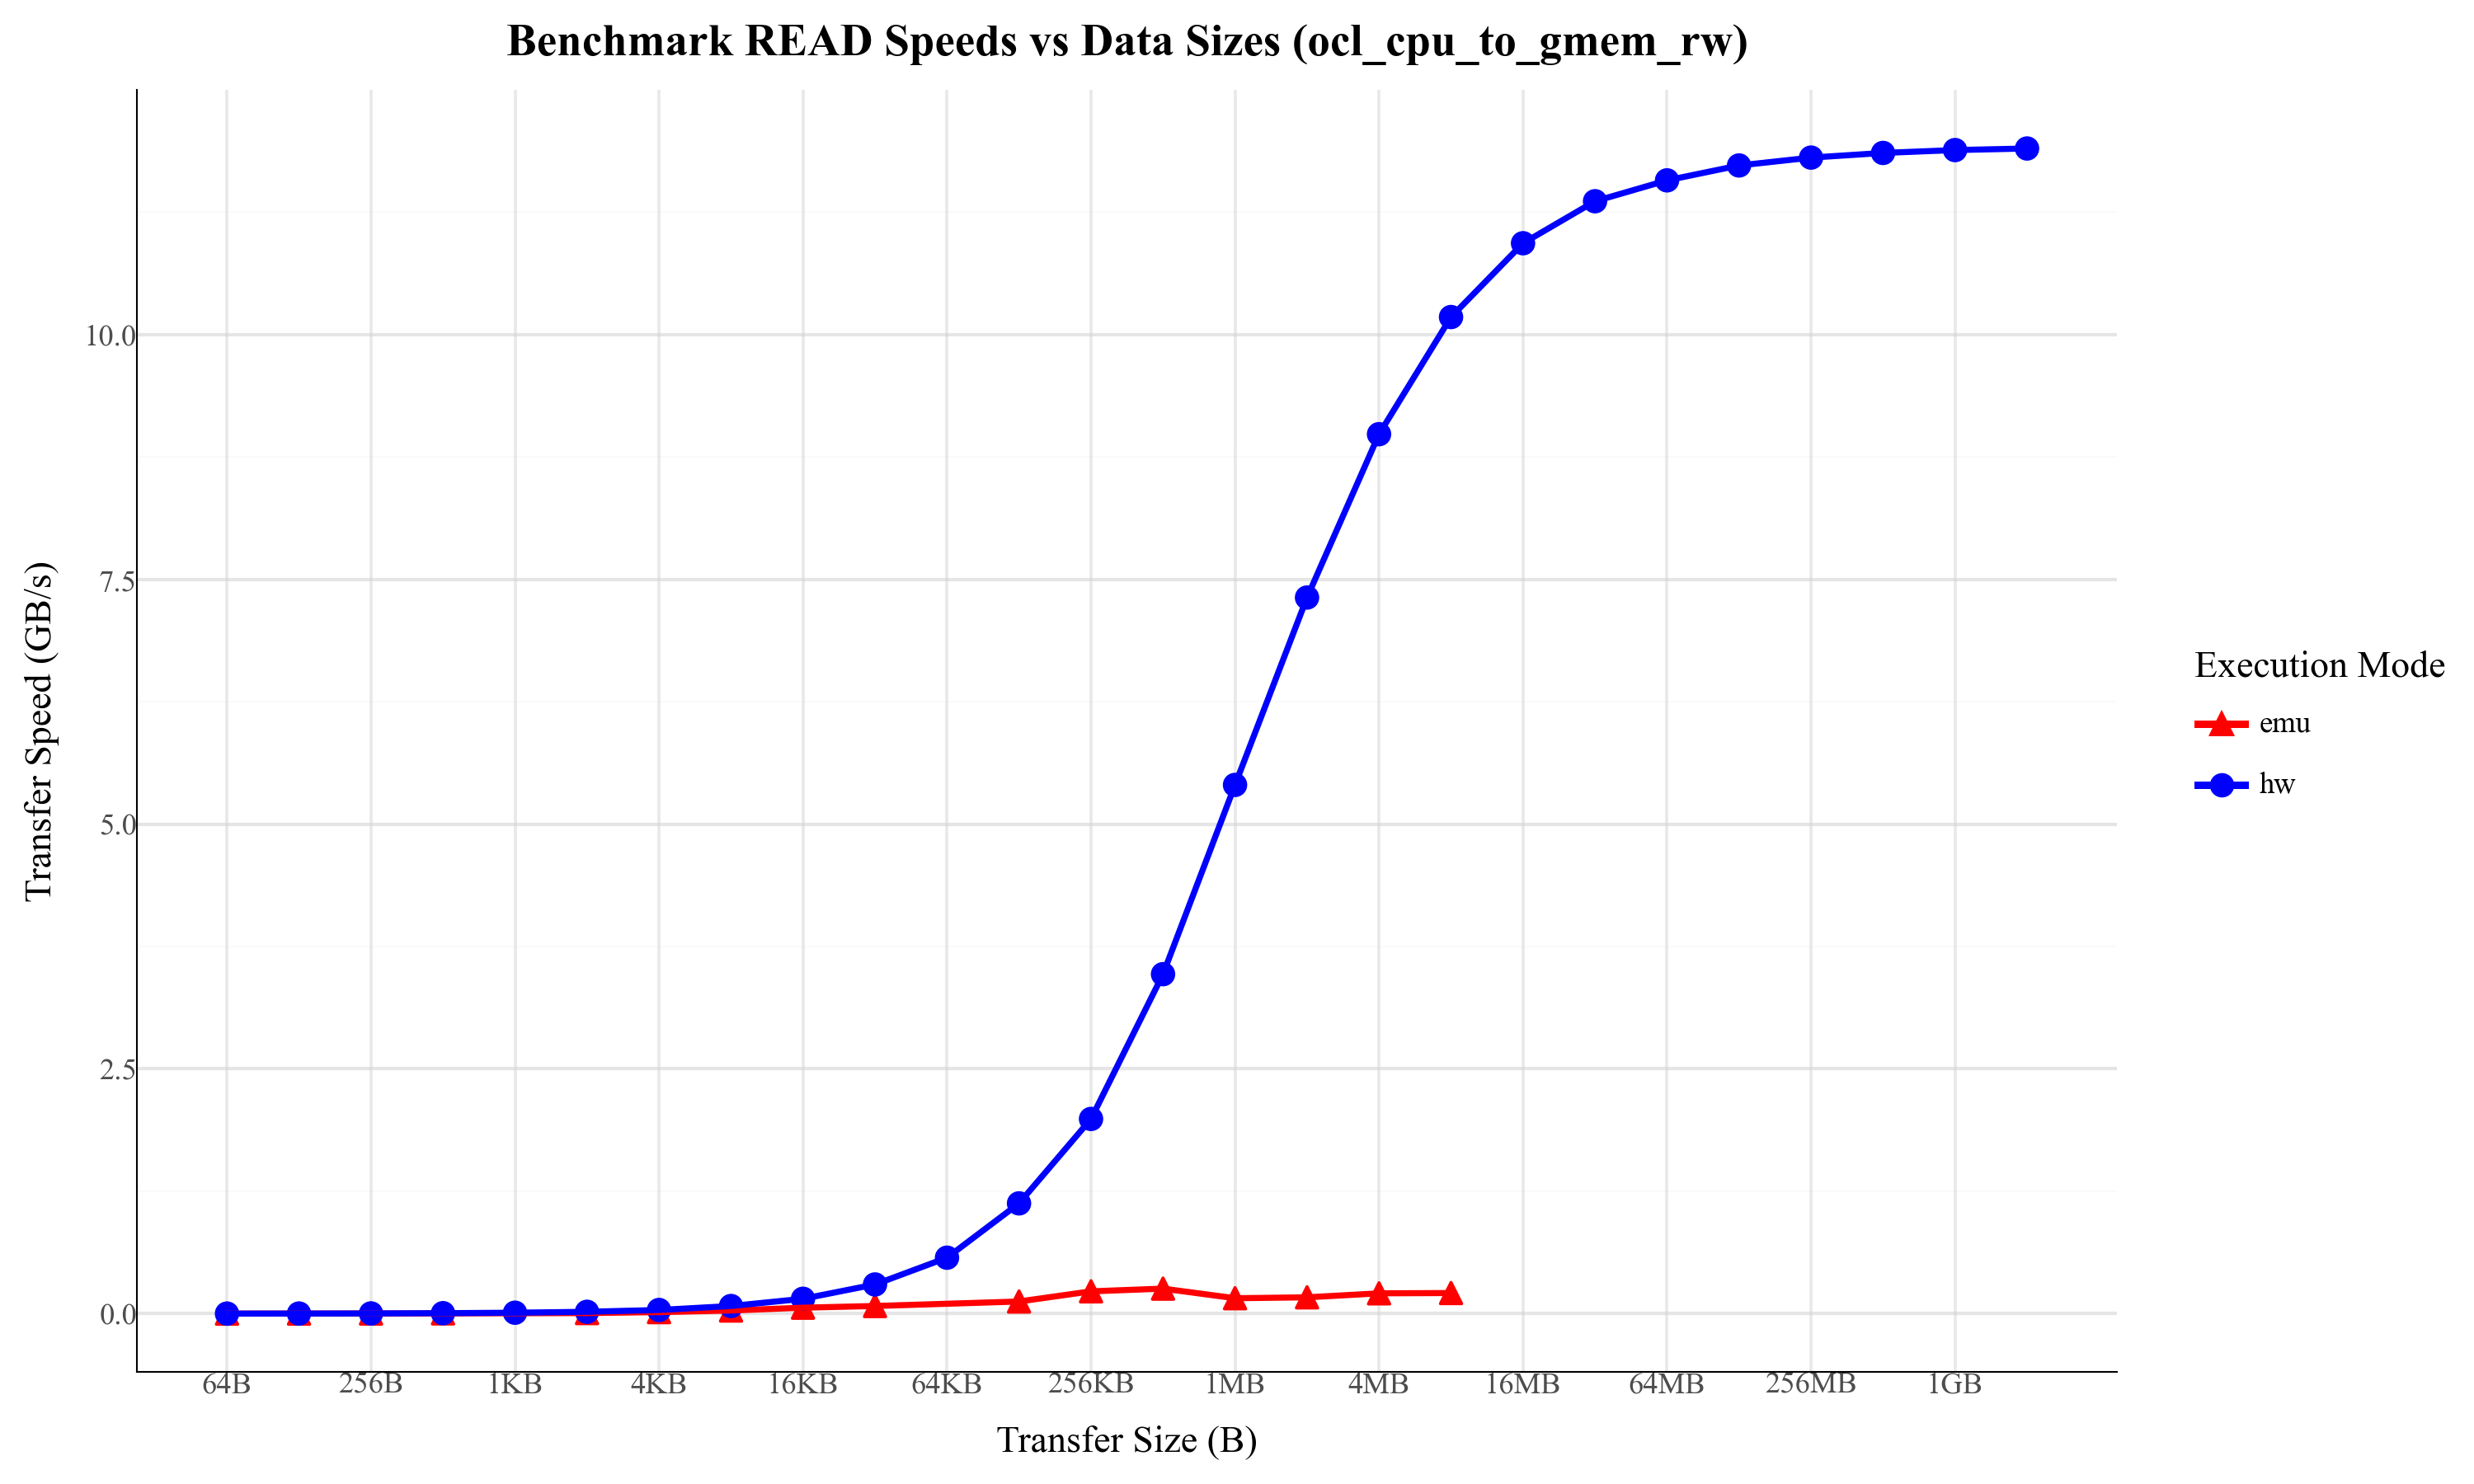
\includegraphics[width=0.9\linewidth]{content/ocl_cpu_to_gmem_rw_READ.png}
    \caption{Log10 Graph of Consecutive Data READ Speeds Comparison from CPU to GMEM for HW and EMU using OCL.}
    \label{fig:enter-label}
\end{figure}

\begin{figure}[H]
    \centering
    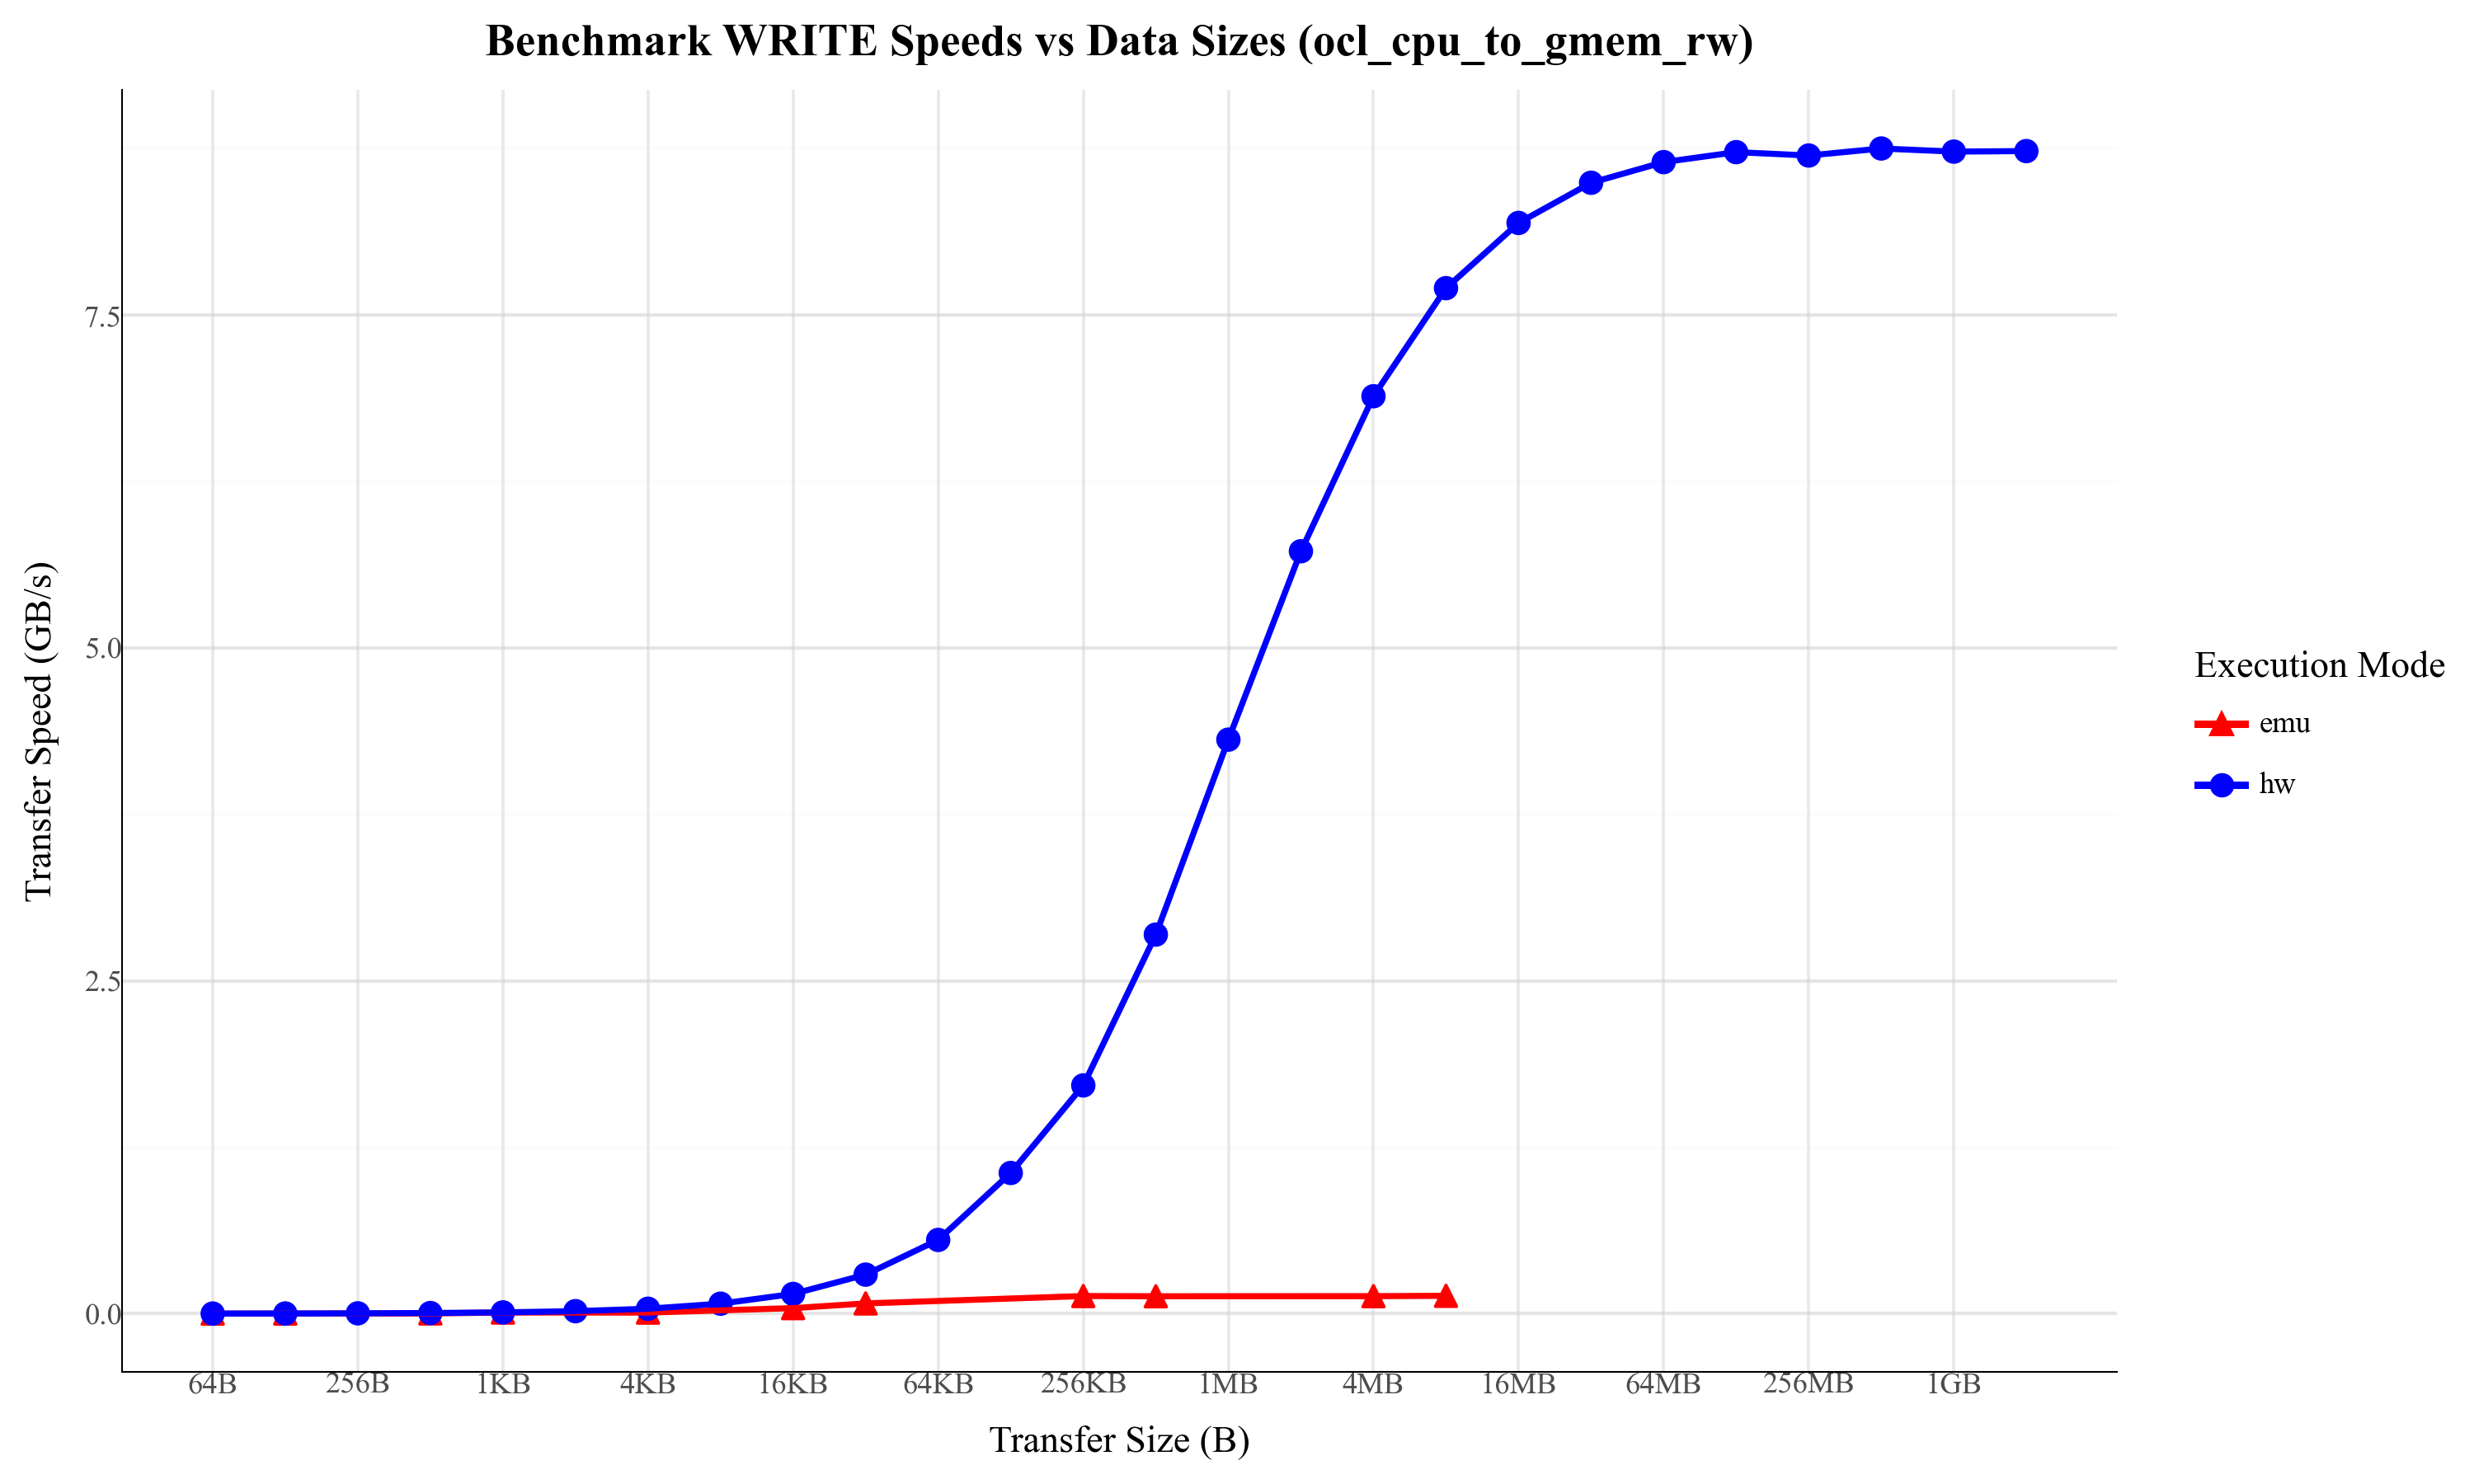
\includegraphics[width=0.9\linewidth]{content/ocl_cpu_to_gmem_rw_WRITE.png}
    \caption{Log10 Graph of Consecutive Data WRITE Speeds Comparison from CPU to GMEM for HW and EMU using OCL.}
    \label{fig:enter-label}
\end{figure}

\begin{figure}[H]
    \centering
    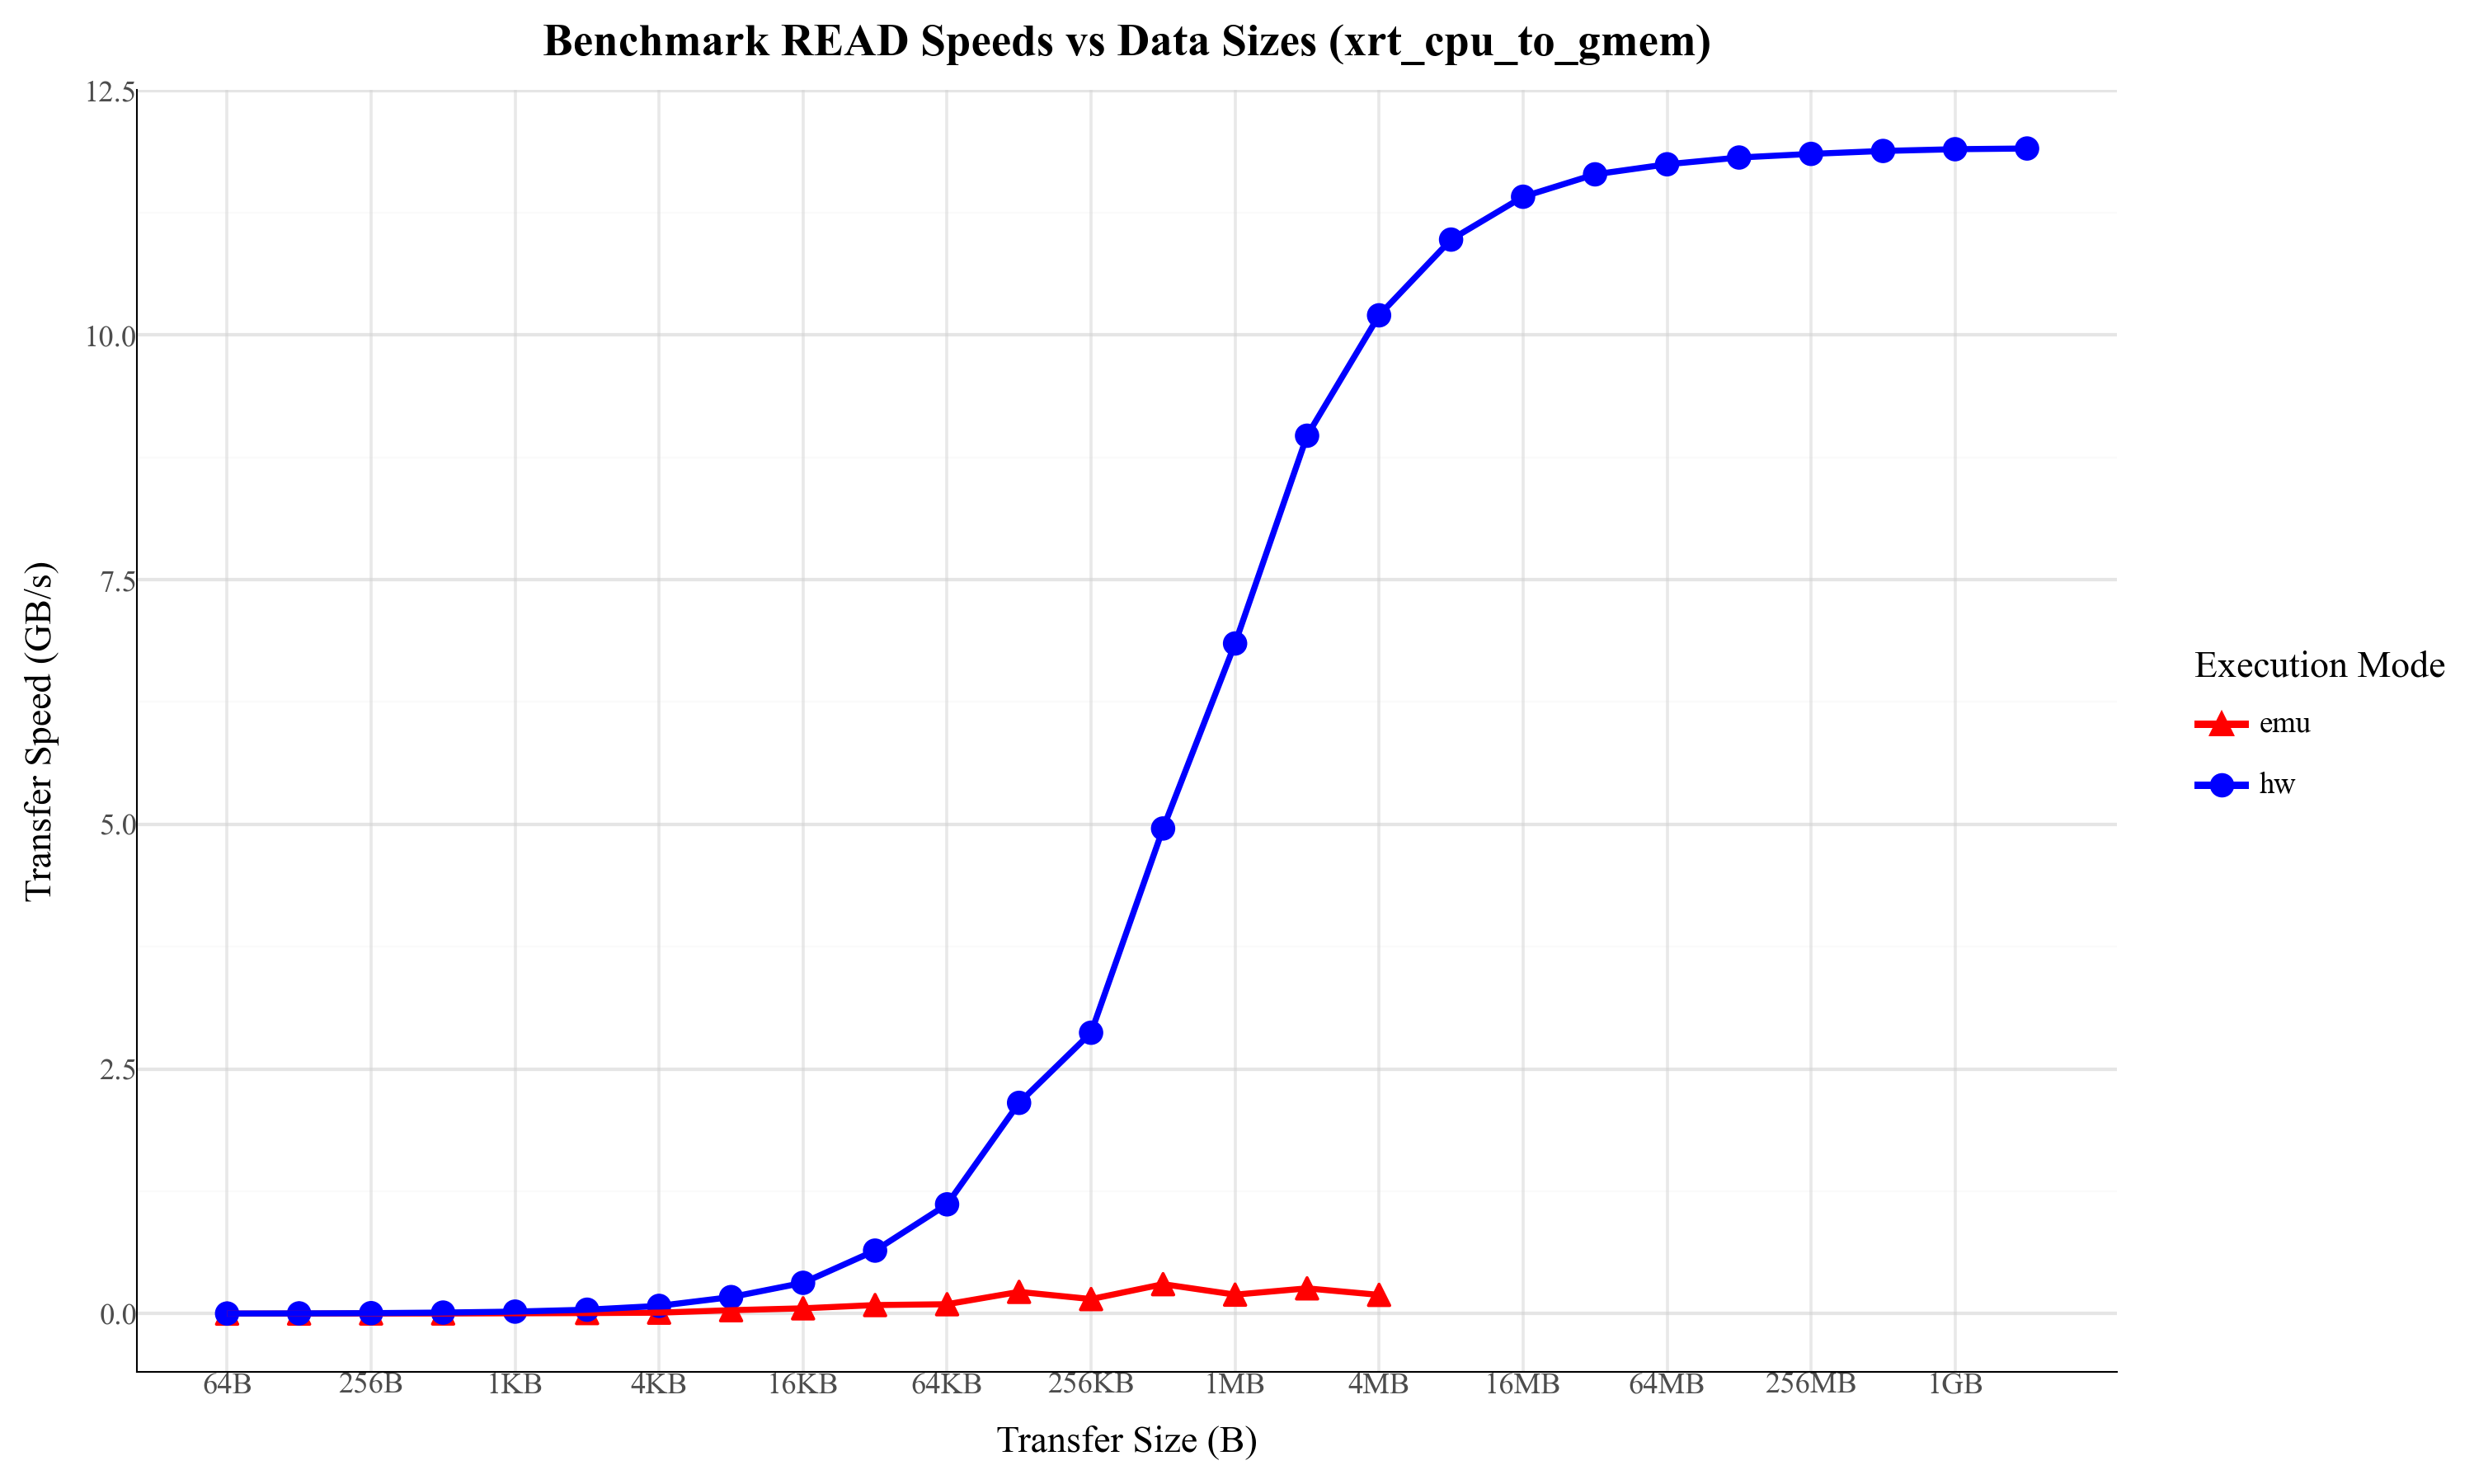
\includegraphics[width=0.9\linewidth]{content/xrt_cpu_to_gmem_READ.png}
    \caption{Log10 Graph of Data READ Speeds Comparison from CPU to GMEM for HW and EMU using XRT API.}
    \label{fig:enter-label}
\end{figure}

\begin{figure}[H]
    \centering
    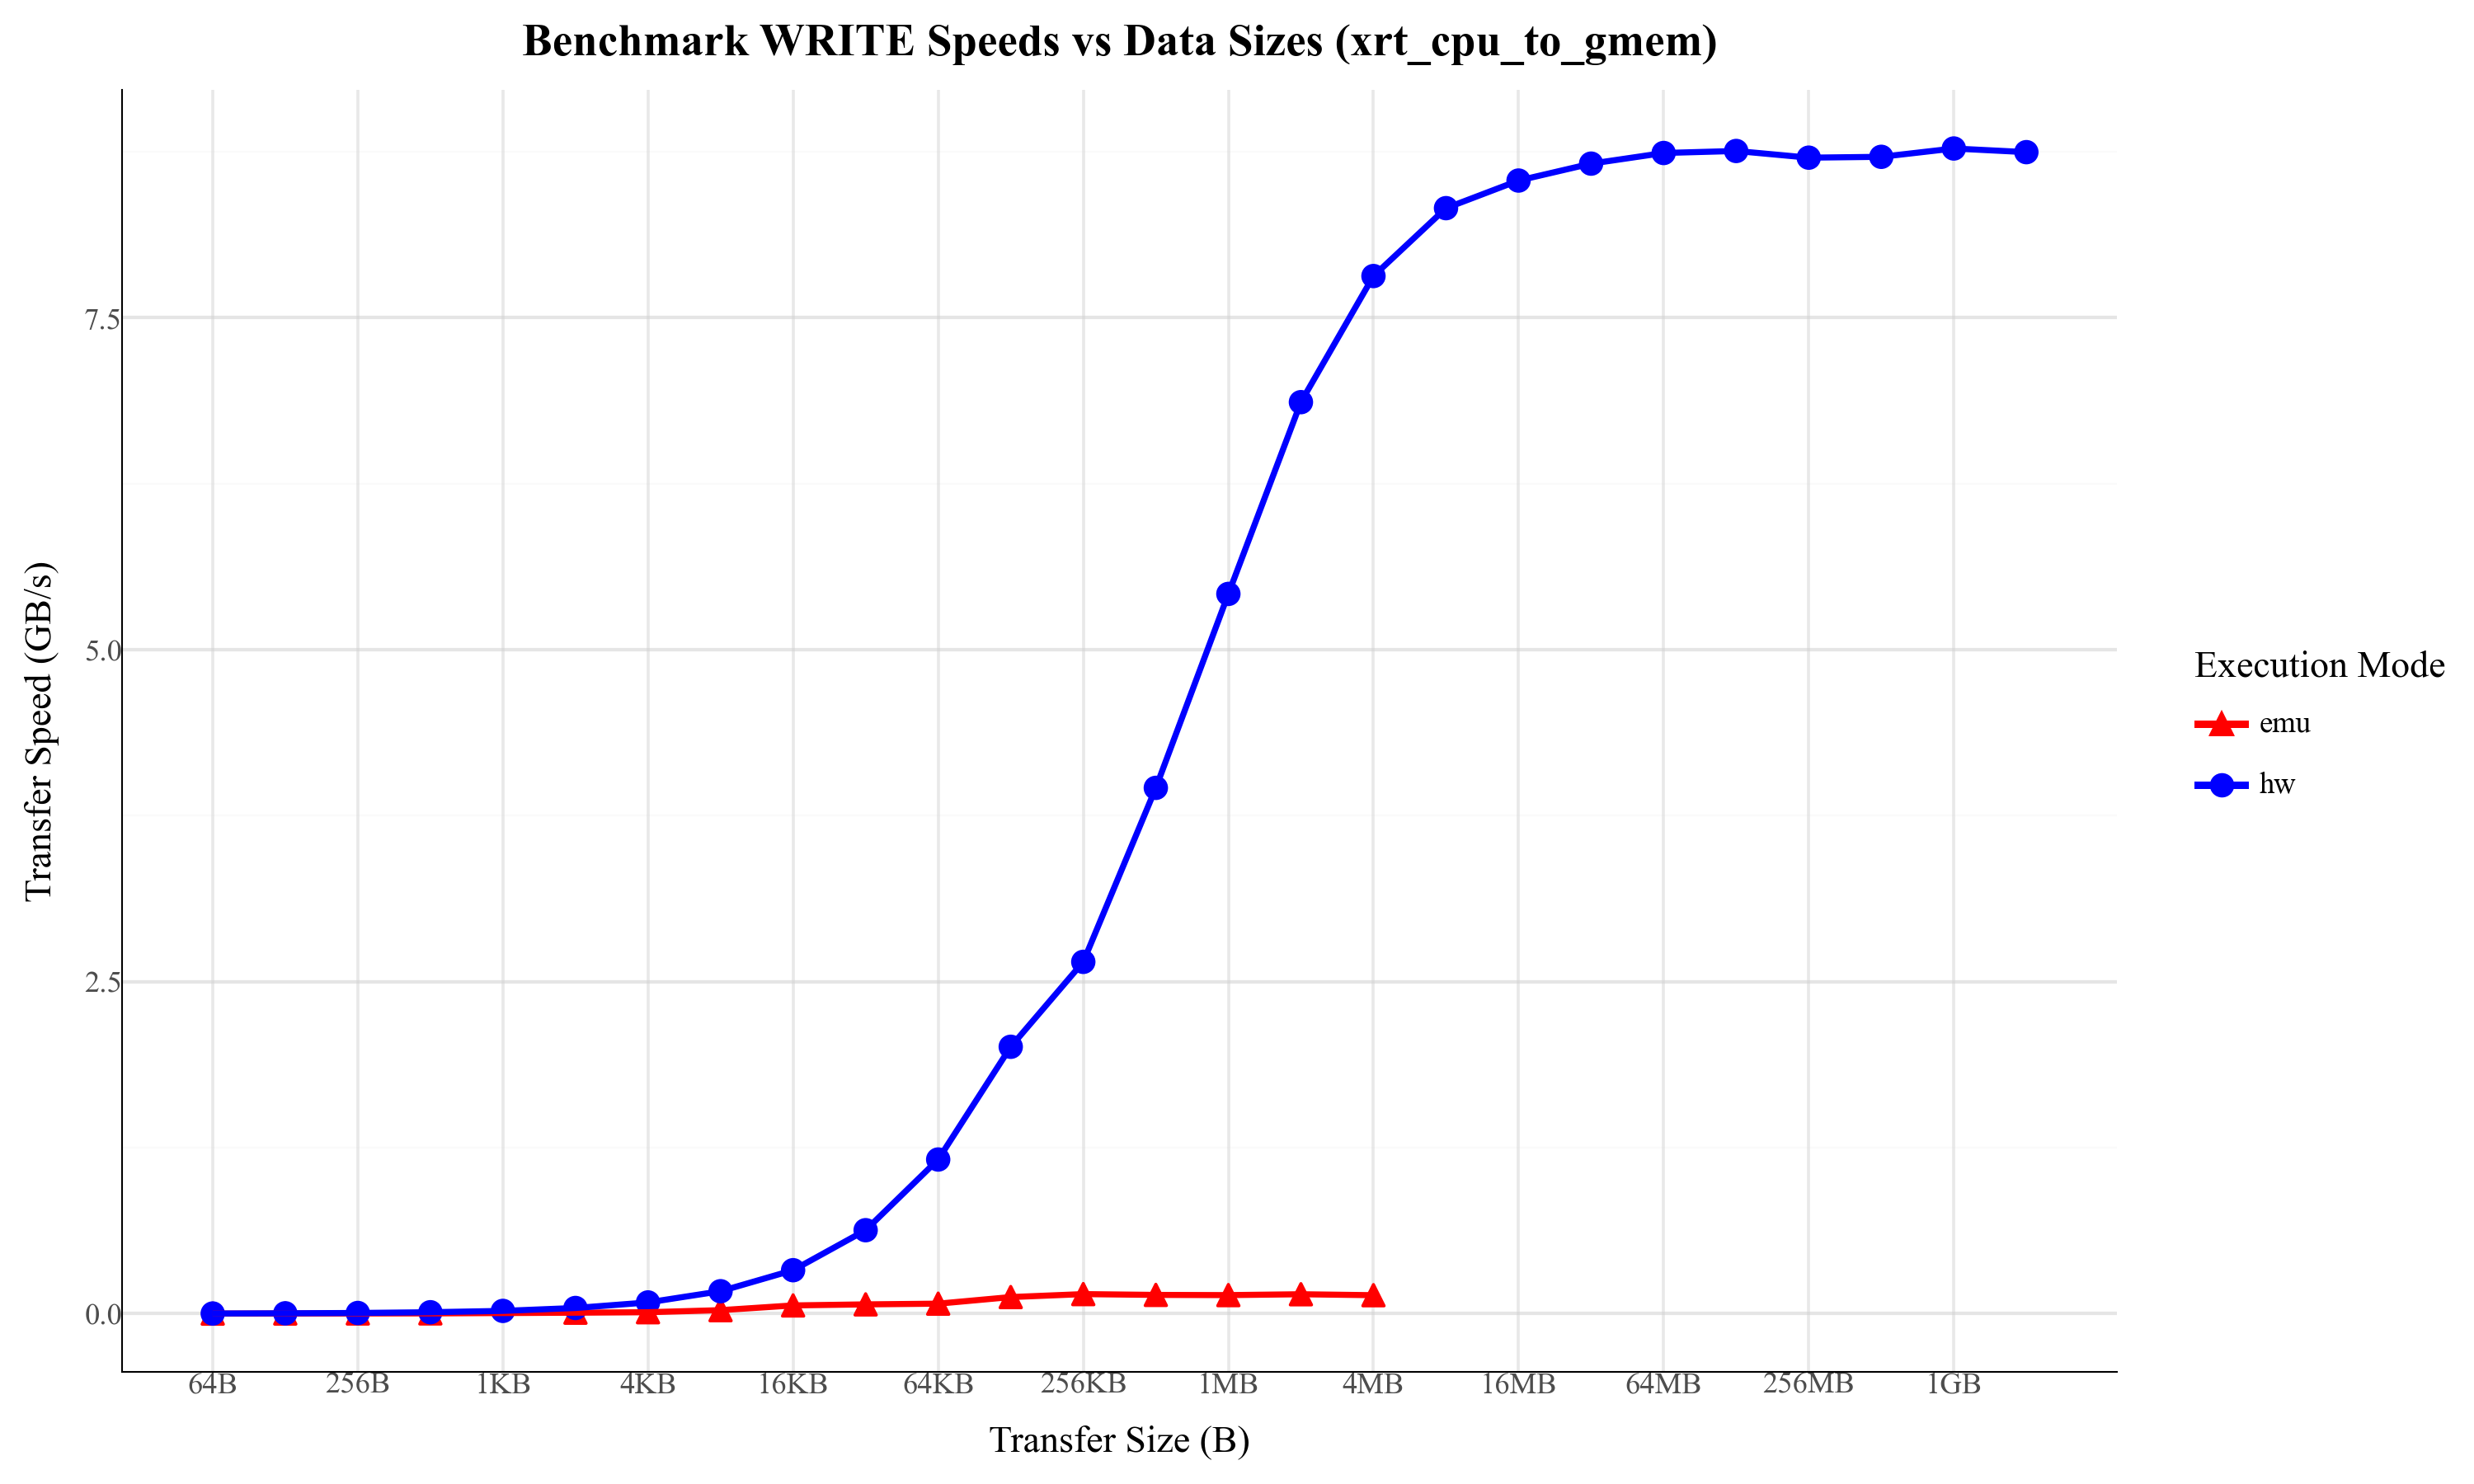
\includegraphics[width=0.9\linewidth]{content/xrt_cpu_to_gmem_WRITE.png}
    \caption{Log10 Graph of Data WRITE Speeds Comparison from CPU to GMEM for HW and EMU using XRT API.}
    \label{fig:enter-label}
\end{figure}

\begin{figure}[H]
    \centering
    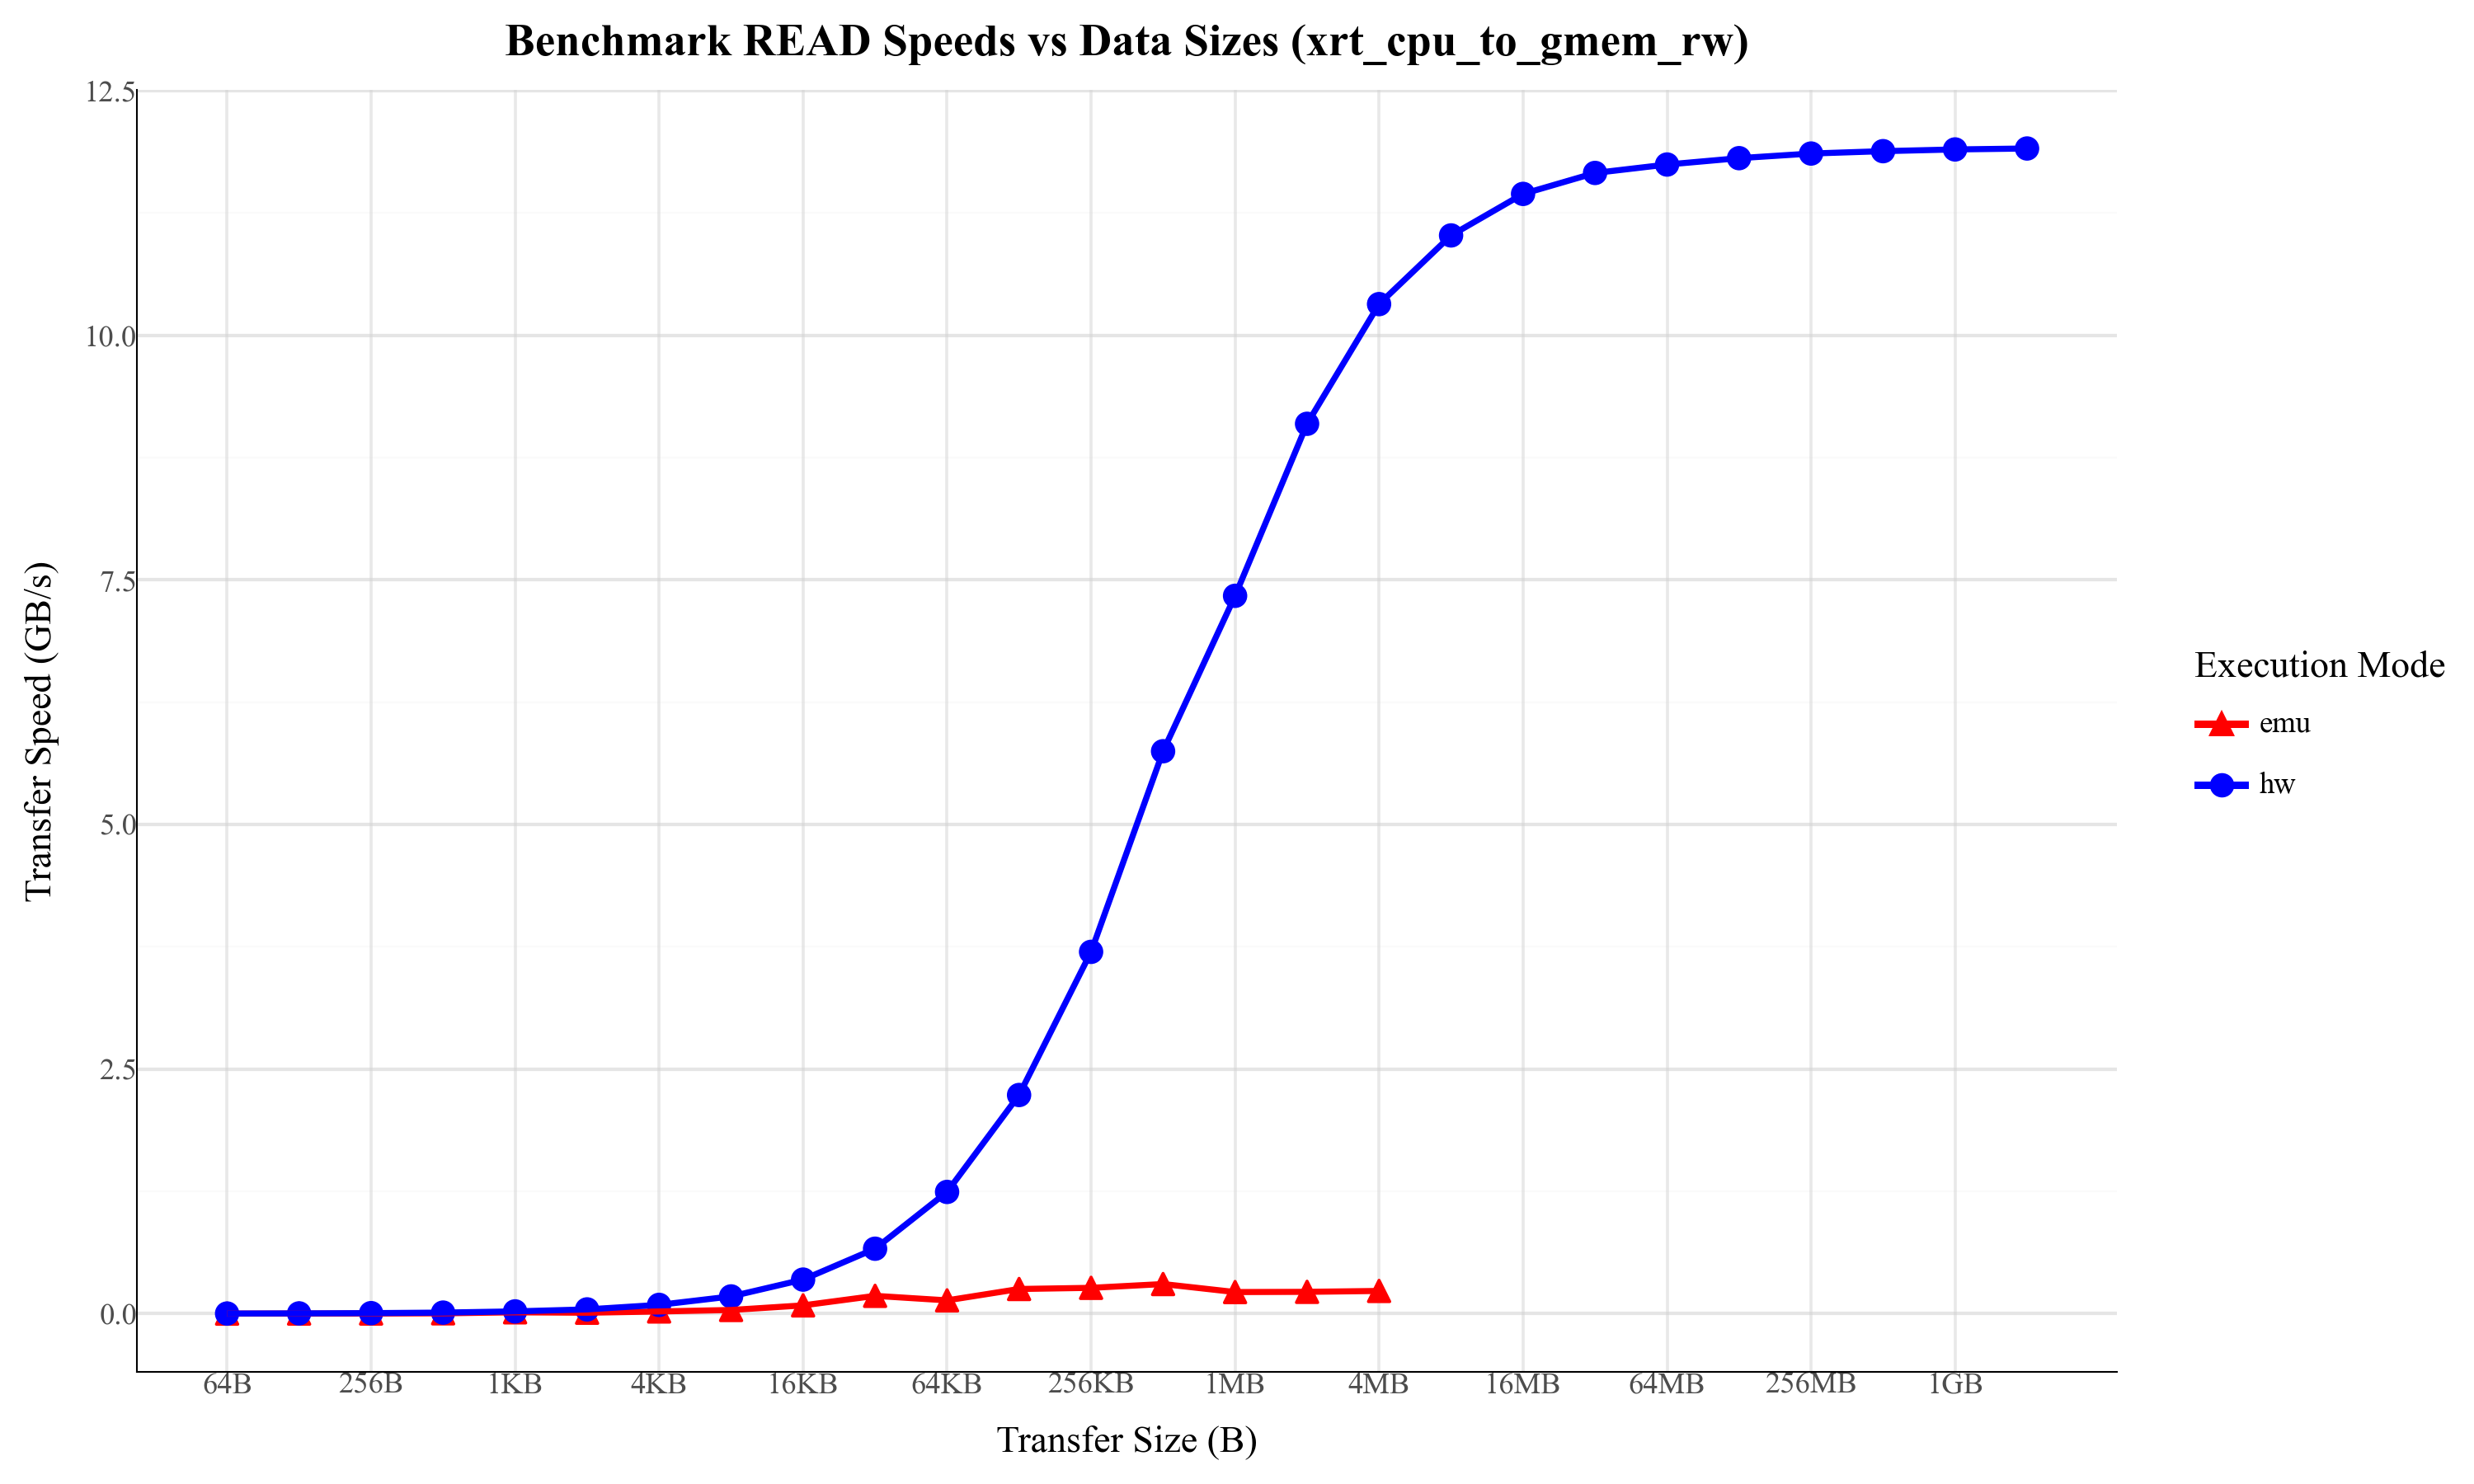
\includegraphics[width=0.9\linewidth]{content/xrt_cpu_to_gmem_rw_READ.png}
    \caption{Log10 Graph of Consecutive Data READ Speeds Comparison from CPU to GMEM for HW and EMU using XRT API.}
    \label{fig:enter-label}
\end{figure}

\begin{figure}[H]
    \centering
    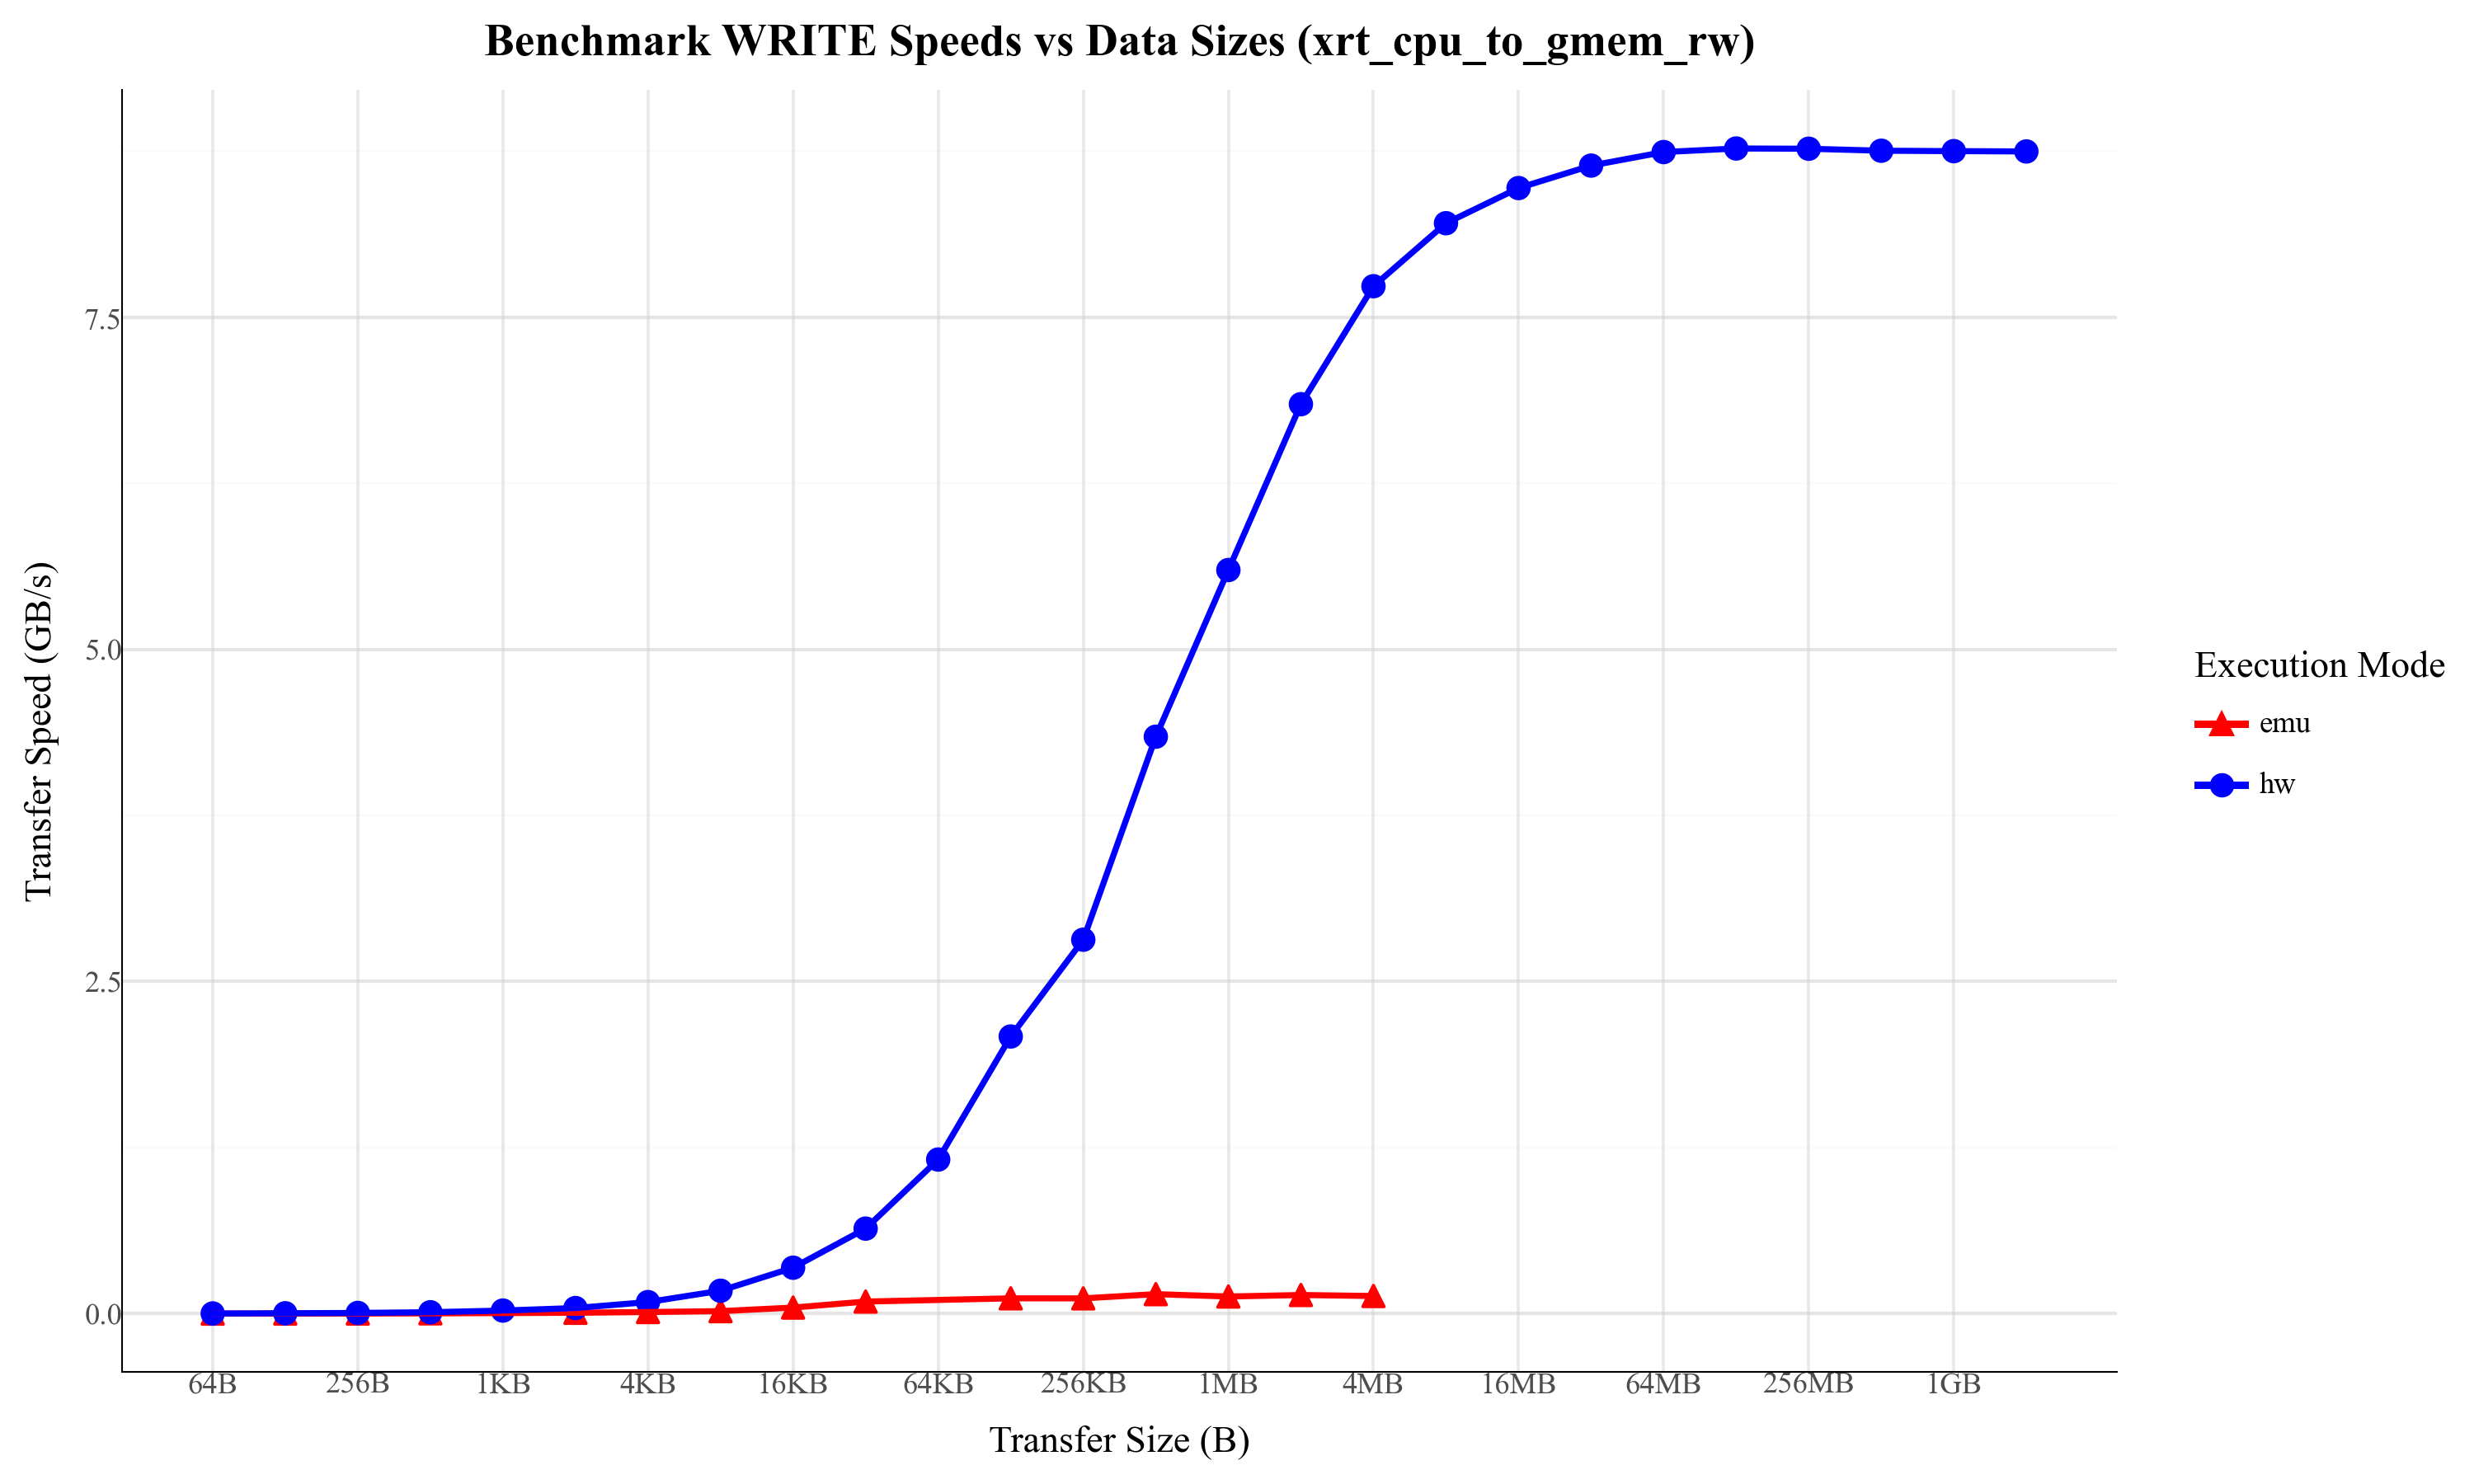
\includegraphics[width=0.9\linewidth]{content/xrt_cpu_to_gmem_rw_WRITE.png}
    \caption{Log10 Graph of Consecutive Data WRITE Speeds Comparison from CPU to GMEM for HW and EMU using XRT API.}
    \label{fig:enter-label}
\end{figure}

% Removed due to lacking support on HW.
% \begin{figure}[H]
%     \centering
%     \includegraphics[width=1.0\linewidth]{content/ocl_fpga_to_gmem_READ.png}
%     \caption{Log10 Graph of Data READ Speeds Comparison from FPGA to GMEM for HW (unsupported) and EMU.}
%     \label{fig:enter-label}
% \end{figure}

% \begin{figure}[H]
%     \centering
%     \includegraphics[width=1.0\linewidth]{content/ocl_fpga_to_gmem_WRITE.png}
%     \caption{Log10 Graph of Data WRITE Speeds Comparison from FPGA to GMEM for HW (unsupported) and EMU.}
%     \label{fig:enter-label}
% \end{figure}
\section{Evaluations}

\subsection{Emulation Results}
At first glance, the transfer rates for all CPU to GMEM methods are slow (less than 1 GB/s). The emulation times are taken directly from the \texttt{summary.csv} and \texttt{native\_trace.csv} provided by Xilinx after the execution of host. As mentioned in the emulation logs, "Hardware emulation runs simulation underneath. Using a large data set will result in long simulation times. It is recommended that a small dataset is used for faster execution." \\

Hardware emulation is significantly slower than actual hardware execution because it simulates the entire hardware system in software, including the intricate details of CPU operations, memory accesses, and data transfers. This software-based simulation must process each operation step-by-step, resulting in a substantial overhead compared to the near-instantaneous execution that occurs on physical hardware. Due to these limitations and resource constraints, emulation tests were run only once and took about a day to compile and execute with large data sets. \\

While there cannot be a accurate comparison due to the degraded performance of hardware emulation, it is still possible to compare relative trends. \\

\begin{table}[H]
    \centering
    \begin{tabular}{c|c}
         Peak READ Speed & 0.259 GB/s @ 512 KB \\
         Peak Consecutive READ Speed & 0.256 GB/s @ 512 KB \\
         Peak WRITE Speed & 0.147 GB/s @ 8 MB \\
         Peak Consecutive WRITE Speed & 0.134 GB/s @ 8 MB \\
    \end{tabular}
    \caption{Notable Emulation Data Transfer Speeds (GB/s) for OCL CPU to GMEM}
    \label{tab:my_label}
\end{table}

\begin{table}[H]
    \centering
    \begin{tabular}{c|c}
         Peak READ Speed & 0.301 GB/s @ 512 KB \\
         Peak Consecutive READ Speed & 0.303 GB/s @ 512 KB \\
         Peak WRITE Speed & 0.147 GB/s @ 256 KB \\
         Peak Consecutive WRITE Speed & 0.147 GB/s @ 512 KB \\
    \end{tabular}
    \caption{Notable Emulation Data Transfer Speeds (GB/s) for XRT CPU to GMEM}
    \label{tab:my_label}
\end{table}

From Table 1 and Table 2, it is clear that in general, the peak WRITE speeds are slower compared to the peak READ speeds. The READ speeds using the XRT API appear to be a bit faster, but there is no obvious difference between the WRITE speeds of the 2 APIs. \\

There does not seem to be a obvious drop in data transfer speeds regarding singular data transfers and consecutive data transfers, except for the WRITE speeds when doing consecutive READ/WRITEs. This is likely due to the additional overhead in using OCL for data transfers. Another trend to notice is that in emulation, after reaching the peak speeds, the transfer data rates seem to drop when a higher data size is being transferred. There does not appear to be a trend regarding when the peak transfer rate is reached for each method. \\

For small data transfers, latency is the most important factor for considering performance. As seen in all the graphs, the latency is low for all small sized data transfers. However, due to the fixed overhead for setting up the transfer, it is still significant. In this case, for small data transfers, around a few bytes, the XRT API shows significant advantage, taking only 3/4 of the time that OCL takes. In this emulation scenario, it is clear that XRT has less data transfer overhead than OCL. 

\subsection{Hardware Results}

While emulation provides insights into system behavior (such as for functional verification), it does not accurately reflect real-world performance. Therefore, the following analysis will focus more on actual hardware results, which offer a more realistic representation of system capabilities. \\

\begin{table}[H]
    \centering
    \begin{tabular}{c|c}
         Peak READ Speed & 11.901 GB/s @ 2.0 GB \\
         Peak Consecutive READ Speed & 11.901 GB/s @ 2.0 GB \\
         Peak WRITE Speed & 8.795 GB/s @ 0.5 GB \\
         Peak Consecutive WRITE Speed & 8.752 GB/s @ 0.5 GB \\
    \end{tabular}
    \caption{Notable Hardware Data Transfer Speeds (GB/s) for OCL CPU to GMEM}
    \label{tab:my_label}
\end{table}

\begin{table}[H]
    \centering
    \begin{tabular}{c|c}
         Peak READ Speed & 11.906 GB/s @ 2.0 GB \\
         Peak Consecutive READ Speed & 11.908 GB/s @ 2.0 GB \\
         Peak WRITE Speed &  8.775 GB/s @ 1.0 GB \\
         Peak Consecutive WRITE Speed & 8.769 GB/s @ 0.125 GB \\
    \end{tabular}
    \caption{Notable Hardware Data Transfer Speeds (GB/s) for XRT CPU to GMEM}
    \label{tab:my_label}
\end{table}

Similarly to the emulation results, according to Table 3 and 4, the peak WRITE speeds are a bit slower than the peak READ speeds. Contrast to emulation results, both APIs display similar peak speed results. This leads to the conclusion that the overhead in OCL is relatively low for large sized data transfers, and does not affect the data transfer speeds in a noticeable way. \\

The data transfer speeds between singular data transfers and consecutive data transfers are also similar for both APIs, leading to the conclusion that sending consecutive data transfers has no noticeable affect on READ/WRITE speeds. Next, hardware results did not see it's data transfer speeds taper off after reaching it's peak data transfer rate but instead seemed to keep a constant data transfer rate after as the data sizes grew. There does not appear to be a trend regarding when the peak transfer rate is reached for each method. \\

Now, analyzing the data transfer speeds for small data sizes. It is shown that XRT shows significant speed advantages, using only 1/3 to 1/2 of the time that OCL takes to transfer. This clearly shows that OCL has more setup overhead compared to XRT, but has less of a impact when data sizes are large enough that the extra time taken is insignificant.
\section{Conclusions}

The emulation tests provided valuable insights into system behavior, but they do not fully capture real-world performance due to significant overhead and slower execution times. While emulation is useful for functional verification, it falls short in accurately reflecting actual hardware performance. The trends observed in hardware tests, such as consistent transfer speeds for large data sizes and similar rates for consecutive transfers, reinforce the reliability of the hardware measurements over emulation results. Therefore, while emulation offers a preliminary understanding, hardware testing is essential for precise performance evaluation. \\

Based on the benchmarking results, it is clear that both OpenCL (OCL) and Xilinx Runtime (XRT) APIs have their own strengths in data transfers. For small data sizes, XRT consistently outperforms OCL due to lower overhead, making it a more efficient choice for minimizing latency. However, for larger data sizes, both APIs achieve similar peak transfer speeds, indicating that OCL's overhead becomes negligible as data size increases. This suggests that while XRT offers an edge in scenarios requiring rapid, small transfers, OCL is equally viable for larger data transfers when peak throughput is the primary concern. \\

These findings have significant implications for FPGA-based application development. Choosing between OpenCL and XRT can greatly impact performance, especially in applications where latency and throughput are critical. For instance, in high-frequency trading, where microseconds matter, the lower overhead of XRT for small data transfers could provide a competitive edge. Similarly, if the data transfers are large and a fast development time is needed, then OCL might be the right choice as it is inherently easier and the overhead becomes negligible. This study aids in making informed decisions, ensuring that the chosen technology aligns with the specific requirements of a given application.

\end{document}